\documentclass[handout]{beamer}
%\documentclass{beamer}
{
\usepackage{fullpage}
\usepackage{hyperref}
\usepackage{amssymb} 
}
\usepackage{pgf,pgfarrows,pgfnodes,pgfautomata,pgfheaps,pgfshade}
\usepackage{amsmath,amscd,amssymb}
\usepackage{colortbl}
\usepackage{tikz,pgf,pifont}
\usepackage{mathtools}
\usepackage{pbox}

\usepackage{lstlisting-llvm}
\usepackage[numbered]{mcode}
\usepackage{listings}
\lstloadlanguages{Matlab}
\lstdefinestyle{mcode}{language=MATLAB,escapechar=&}

\usepackage{xcolor}
\usepackage{textcomp}
\usepackage{pgfpages}
\usepackage{hologo}

%\pgfpagesuselayout{4 on 1}[a4paper, border shrink=5mm, landscape]



%\usepackage[latin1]{inputenc}
\usepackage[english]{babel}

  \usetheme{Boadilla}    % Very nice with fewer sections/sub and numbering
  % \usetheme{CambridgeUS}  % Sections and red white + numbers
  % \usetheme{Warsaw}      % Good one no numbers though
  % \usetheme{Darmstadt}   % no University and name
   \setbeamercovered{transparent}
  % \useoutertheme[subsection=true,footnote=false]{miniframes}
  \setbeamertemplate{navigation symbols}{}
  \usecolortheme{crane}

\usepackage{amsmath, amssymb, amsfonts, amsthm,
  verbatim, fancyhdr, graphicx, array, latexsym,
  color, listings, afterpage, epsfig, boxedminipage, 
  fancybox}
\usepackage{amsfonts,amsbsy}


%\usepackage[emtex]{changebar}
%\usepackage{mathptm}  % times+ math
%\usepackage{natbib}
%\usepackage{epsf}
%\usepackage{epsfig}
%\usepackage{rotate}
%\usepackage{amsmath}
%\usepackage{ifthen}
%\usepackage[english]{babel}
% or whatever
%\usepackage[latin1]{inputenc}

% or whatever 
\newcommand{\ud}{\mathrm{d}}
\newcommand{\commentout}[1]{}
\newcommand{\mybox}[1]{\hbox to 0.6\textwidth{#1\hss}}
\newcommand{\pmat}[1]{\begin{pmatrix}#1\end{pmatrix}} 
\newcommand{\red}[1]{\textcolor{red}{#1}}
\newcommand{\blue}[1]{\textcolor{blue}{#1}}
\newcommand{\brown}[1]{\textcolor{brown}{#1}}
\newcommand{\green}[1]{\textcolor{green}{#1}}
\newcommand{\purple}[1]{\textcolor{purple}{#1}}
\newcommand{\gray}[1]{\textcolor{gray}{#1}}


\newcommand{\pder}[2]{\frac{\partial #1}{\partial #2}}
 \newcommand{\norm}[2]{\ensuremath{\| #1 \|_{#2}}}
 \newcommand{\seq}[1]{\ensuremath{\left\{ #1 \right\}}}
 \newcommand{\ipt}[2]{\ensuremath{\left\langle#1,#2\right\rangle}}
 \newcommand{\vbblock}[3]{\ensuremath{\left(\begin{array}{c}\!\!\!#1\\\!\!\!#2\\\!\!\!#3\end{array}\!\!\!\right)}}

 \newcommand{\bblock}[9]{\ensuremath{\left(\begin{array}{ccc}#1&#2&#3\\#4&#5&#6\\#7&#8&#9\end{array}\right)}}
 \def \R{\bb{R}}\def \C{\bb{C}}\def \Z{\bb{Z}}\def \N{\bb{N}}
 \def \a{{\bf a}}
 \def \b{{\bf b}}
 \def \c{{\bf c}}
 \def \d{{\bf d}}
 \def \e{{\bf e}}
 \def \f{{\bf f}}
 \def \g{{\bf g}}
 \def \k{{\bf k}}
 \def \m{{\bf m}}
 \def \n{{\bf n}}
 \def \p{{\bf p}}
 \def \q{{\bf q}}
 \def \r{{\bf r}}
 \def \s{{\bf s}}
 \def \t{{\bf t}}
 \def \u{{\bf u}}
 \def \vv{{\bf v}}
 \def \w{{\bf w}}
 \def \x{{\bf x}}
 \def \y{{\bf y}}
 \def \z{{\bf z}}
 \def \rh{{\alert{h}}}
\def \M{{\cal M}}
\def \L{{\cal L}}
 \def \blambda{{\boldsymbol{\lambda}}}%works with package amsbsy
\newcommand{\hnorm}[2]{\ensuremath{| #1 |_{#2}}}
\newcommand{\ip}[2]{\ensuremath{\left(#1,#2\right)}}




\definecolor{Brown}{cmyk}{0,0.81,1,0.60}
\definecolor{Green}{rgb}{0.516, 0.5976, 0.480}
\definecolor{OliveGreen}{cmyk}{0.64,0,0.95,0.40}
\definecolor{CadetBlue}{rgb}{0.17,0.30,0.547}
\definecolor{Red}{rgb}{0.684,0.156,0.32}
\lstset{
  language=matlab,
  basicstyle=\ttfamily,
  frame=ltrb,
  framesep=5pt,
  basicstyle=\scriptsize,
  stringstyle=\ttfamily\color{Brown}\bfseries,
  commentstyle=\ttfamily\color{Green}\bfseries,
  keywordstyle=\ttfamily\color{CadetBlue}\bfseries,
  identifierstyle=\ttfamily, 
  tabsize=2,
  showstringspaces=true,
  numbers=none
}




%%%%%%%%%%%%%%%%%%%%%%%%%%%%%%%%%%%%%%%%%%%%%%%%%%%%%%%%%%%%%%%%%%%%%%
%%%%%%%%%%%%%%%%%%%%%%%%%%%%%%%%%%%%%%%%%%%%%%%%%%%%%%%%%%%%%%%%%%%%%%
%%%%%%%%%%%%%%%%%%%%%%%%%%%%%%%%%%%%%%%%%%%%%%%%%%%%%%%%%%%%%%%%%%%%%%

% slide 1:
% ========

% title and affiliation

\title[PDE LAB6, 2015]{Master of Science on Computational Science}



\author[prof. Dr. Rolf Krause \& Dr. Drosos Kourounis] % (optional, use only with lots of authors)
{\textbf{Institute of Computational Science}}
% - Give the names in the same order as the appear in the paper.
% - Use the \inst{?} command only if the authors have different
%   affiliation.

\institute[ICS] % (optional, but mostly needed)
{
prof. Dr. Rolf Krause \& Dr. Drosos Kourounis
}
% If you have a file called "university-logo-filename.xxx", where xxx
% is a graphic format that can be processed by latex or pdflatex,
% resp., then you can add a logo as follows:


%\pgfdeclareimage[height=1.0cm]{university-logo}{uoi}
%\logo{\pgfuseimage{university-logo}}

% - Use the \inst command only if there are several affiliations.
% - Keep it simple, no one is interested in your street address.

\date[22 Oct, 2015]{22 Oct 2015, LAB6}

\usefonttheme{serif}


\AtBeginSubsection[]
{
  \begin{frame}<beamer>
    \frametitle{Outline}
    \tableofcontents[currentsection,currentsubsection]
  \end{frame}
}
\setbeamertemplate{footline}
{
  \begin{beamercolorbox}[colsep=1.5pt]{upper separation line foot}
  \end{beamercolorbox}
  \begin{beamercolorbox}[ht=2.5ex,dp=1.125ex,%
    leftskip=.3cm,rightskip=.3cm plus1fil]{title in head/foot}%
    \leavevmode{\usebeamerfont{title in head/foot}
      \insertsection \hfill \insertsubsection\ \hfill \insertshorttitle}%
  \end{beamercolorbox}%
  \begin{beamercolorbox}[colsep=1.5pt]{lower separation line foot}
  \end{beamercolorbox}
}



\begin{document}


\begin{frame}
  \titlepage
\end{frame}

\section{Finite Elements for 3D tetrahedra}



\begin{frame}{The 3D reference tetrahedral element}
\begin{minipage}{0.45\textwidth}
\begin{figure}
     \begin{picture}(180,95)(-50,0)
     \thicklines
     \put(0,0){\line(1, 0){80}}
%     \put(80,0){\line(0, 1){80}}
%     \put(80,80){\line(-1, 0){80}}
     \put(80,0){\line(-1, 1){80}}
     \put(0,0){\line(0, 1){80}}
     \put(0,0){\line(-1, -1){52}}
     \put(0,80){\line(-2,-5){53}}
     \put(80,0){\line(-5,-2){133}}
     
     \put(7,3){1}
     \put(60,5){3}
     \put(3,60){4}
     \put(-31,-40){2}


     \put(10,15){\vector(1, 0){30}}
     \put(10,15){\vector(0, 1){30}}
     \put(10,15){\vector(-1, -1){20}}
     \put(10,50){$\zeta$}
     \put(43,15){$\eta$}
     \put(-15,5){$\xi$}

     \put(-5,-15){(0,0,0)}
     \put(70,-15){(0,1,0)}
     \put(-15,90){(0,0,1)}
     \put(-50,-65){(1,0,0)}
     \end{picture}
\end{figure}
\end{minipage}
\begin{minipage}{0.45\textwidth}
\begin{align*}
N_1 &= (1 - \xi - \eta - \zeta) \\
N_2 &= \xi \\ 
N_3 &= \eta \\
N_4 &= \zeta \\
\end{align*}
\end{minipage}
\end{frame}


\begin{frame}{The affine mapping}
The mapping from the reference triangle $T_0$ to the current
triangle $T_e$ with coordinates $(x_0,y_0,z_0),(x_1,y_1,z_1),(x_2,y_2,z_2),(x_3,y_3,z_3)$ is 
\begin{align*}
x   &= x_0 + (x_1 - x_0) \xi + (x_2 - x_0) \eta  + (x_3 - x_0) \zeta \\
y   &= y_0 + (y_1 - y_0) \xi + (y_2 - y_0) \eta  + (y_3 - y_0) \zeta \\
z   &= z_0 + (z_1 - z_0) \xi + (z_2 - z_0) \eta  + (z_3 - z_0) \zeta. 
\end{align*}
Now for any function $f(x,y,z)=f(x(\xi, \eta, \zeta),y(\xi, \eta, \zeta),z(\xi, \eta, \zeta))$ using the 
chain rule of differentiation, we have
\begin{align*}
\pder{f}{\xi}   &= \pder{f}{x}\pder{x}{\xi} + \pder{f}{y}\pder{y}{\xi} + \pder{f}{z}\pder{z}{\xi}\\
\pder{f}{\eta}  &= \pder{f}{x}\pder{x}{\eta} + \pder{f}{y}\pder{y}{\eta} + \pder{f}{z}\pder{z}{\eta} \\
\pder{f}{\zeta}  &= \pder{f}{x}\pder{x}{\zeta} + \pder{f}{y}\pder{y}{\zeta} + \pder{f}{z}\pder{z}{\zeta} \\
\end{align*}

\end{frame}

\begin{frame}{From the current to the reference}
or in more compact form
\begin{align*}
J=
\pmat{ \pder{x}{\xi}  & \pder{y}{\xi} & \pder{z}{\xi}\\ \\
       \pder{x}{\eta} & \pder{y}{\eta} & \pder{z}{\eta}\\ \\
       \pder{x}{\zeta} & \pder{y}{\zeta} & \pder{z}{\zeta}
}
& \quad
dx  dy  dz = |J|\; d\xi  d\eta  d\zeta
\end{align*}

Even more compact, when we differentiate we should keep in mind
\begin{align*}
\nabla_{\boldsymbol \xi} &= J \ \nabla_{\bf x}\\
\nabla_{\bf x} &= J^{-1} \ \nabla_{\boldsymbol \xi}
\end{align*}


\end{frame}

\begin{frame}{The entries of the matrix $J$}
We can map a point $(\xi,\eta,\zeta)$ in the reference tetrahedron
to the point $(x,y,z)$ in the current tetrahedron using the 
equations 
\begin{align*}
x   &= x_0 + (x_1 - x_0) \xi + (x_2 - x_0) \eta + (x_3 - x_0) \zeta\\
y   &= y_0 + (y_1 - y_0) \xi + (y_2 - y_0) \eta + (y_3 - y_0) \zeta \\
z   &= z_0 + (z_1 - z_0) \xi + (z_2 - z_0) \eta + (z_3 - z_0) \zeta. 
\end{align*}
Then it is easy to see that the entries of the Jacobian of $J$ are
\begin{align*}
J=
\pmat{ \pder{x}{\xi}   & \pder{y}{\xi}   & \pder{z}{\xi} \\ \\
       \pder{x}{\eta}  & \pder{y}{\eta}  & \pder{z}{\eta} \\ \\
       \pder{x}{\zeta} & \pder{y}{\zeta} & \pder{z}{\zeta}
}
 = \pmat{ x_1 - x_0 & y_1 - y_0 & z_1 - z_0 
 \\ \\ 
          x_2 - x_0 & y_2 - y_0 & z_2 - z_0
 \\ \\
          x_3 - x_0 & y_3 - y_0 & z_3 - z_0}
\end{align*}

\end{frame}


\begin{frame}{The tetrahedral element using barycentric coordinates}
%$N_i^e &= a^e_i x + b^e_i y + c^e_i$
\centering
\scriptsize
\begin{minipage}{0.45\textwidth}
\begin{align*}
a^e_1 x_1^e + b^e_1 y_1^e + c^e_1 z_1^e + d^e_1 &= 1   \\
a^e_1 x_2^e + b^e_1 y_2^e + c^e_1 z_2^e + d^e_1 &= 0   \\
a^e_1 x_3^e + b^e_1 y_3^e + c^e_1 z_3^e + d^e_1 &= 0   \\
a^e_1 x_4^e + b^e_1 y_4^e + c^e_1 z_4^e + d^e_1 &= 0 
\end{align*}
\end{minipage}
\begin{minipage}{0.45\textwidth}
\begin{align*}
a^e_2 x_1^e + b^e_2 y_1^e + c^e_2 z_1^e + d^e_2 &= 0   \\
a^e_2 x_2^e + b^e_2 y_2^e + c^e_2 z_2^e + d^e_2 &= 1   \\
a^e_2 x_3^e + b^e_2 y_3^e + c^e_2 z_3^e + d^e_2 &= 0   \\
a^e_2 x_4^e + b^e_2 y_4^e + c^e_2 z_4^e + d^e_2 &= 0  
\end{align*}
\end{minipage}
\begin{minipage}{0.45\textwidth}
\begin{align*}
a^e_3 x_1^e + b^e_3 y_1^e + c^e_3 z_1^e + d^e_3 &= 0   \\
a^e_3 x_2^e + b^e_3 y_2^e + c^e_3 z_2^e + d^e_3 &= 0   \\
a^e_3 x_3^e + b^e_3 y_3^e + c^e_3 z_3^e + d^e_3 &= 1   \\
a^e_3 x_4^e + b^e_3 y_4^e + c^e_3 z_4^e + d^e_3 &= 0  
\end{align*}
\end{minipage}
\begin{minipage}{0.45\textwidth}
\begin{align*}
a^e_4 x_1^e + b^e_4 y_1^e + c^e_4 z_1^e + d^e_4 &= 0   \\
a^e_4 x_2^e + b^e_4 y_2^e + c^e_4 z_2^e + d^e_4 &= 0   \\
a^e_4 x_3^e + b^e_4 y_3^e + c^e_4 z_3^e + d^e_4 &= 0   \\
a^e_4 x_4^e + b^e_4 y_4^e + c^e_4 z_4^e + d^e_4 &= 1  
\end{align*}
\end{minipage}

\bigskip

\begin{minipage}{0.65\textwidth}
\begin{align*}
\pmat{x^e_1 & y^e_1 & z^e_1 & 1     \\
      x^e_2 & y^e_2 & z^e_2 & 1     \\
      x^e_3 & y^e_3 & z^e_3 & 1     \\
      x^e_4 & y^e_4 & z^e_4 & 1     \\
} 
\pmat{a^e_1 & a^e_2 & a^e_3 & a^e_4 \\
      b^e_1 & b^e_2 & b^e_3 & b^e_4 \\
      c^e_1 & c^e_2 & c^e_3 & c^e_4 \\
      d^e_1 & d^e_2 & d^e_3 & d^e_4 \\
}
=
\pmat{1     & 0     & 0  & 0   \\
      0     & 1     & 0  & 0   \\
      0     & 0     & 1  & 0   \\
      0     & 0     & 0  & 1   \\
}
\end{align*}
\end{minipage}



\end{frame}


\begin{frame}{The 3D tetrahedral element}
\centering
\begin{minipage}{0.65\textwidth}
\begin{align*}
\pmat{a^e_1 & a^e_2 & a^e_3 & a^e_4 \\
      b^e_1 & b^e_2 & b^e_3 & b^e_4 \\
      c^e_1 & c^e_2 & c^e_3 & c^e_4 \\
      d^e_1 & d^e_2 & d^e_3 & d^e_4 \\
}
=
\pmat{x^e_1 & y^e_1 & z^e_1 & 1     \\
      x^e_2 & y^e_2 & z^e_2 & 1     \\
      x^e_3 & y^e_3 & z^e_3 & 1     \\
      x^e_4 & y^e_4 & z^e_4 & 1     \\
}^{-1} 
\end{align*}
\end{minipage}

\bigskip

\begin{minipage}{0.45\textwidth}
\begin{block}{Barycentric coordinates}
$N_i^e = a^e_i x + b^e_i y + c^e_i z + d^e_i$
\end{block}
\end{minipage}

\bigskip

\begin{minipage}{\textwidth}
\begin{block}{Local approximation}
$u^e(x,y,z) = u^e_1 N^e_1(x,y,z) + u^e_2 N^e_2(x,y,z) + u^e_3 N^e_3(x,y,z) + u^e_4 N^e_4(x,y,z)$
\end{block}
\end{minipage}

\end{frame}


\begin{frame}{Local mass matrix}
\centering
\begin{minipage}{0.65\textwidth}

\begin{block}{Integration on a simplex}
\begin{align*}
\int_{V_e} N_1^i N_2^j N_3^k N_4^l d V_e = \frac{i! j! k! l!}{(d + i + j + k + l!)!} d! V_{e}
\end{align*}
\end{block}

\bigskip 

\begin{block}{Local mass matrix}
\begin{align*}
M_{ij}^e = \int_{V_e} N_i^e N_j^e d V_e = 
\begin{cases}
\frac{V_e}{20}, \quad i \ne j  \\
\frac{V_e}{10}, \quad i = j  
\end{cases}
\end{align*}
\end{block}
%\begin{block}{Mass matrix}
%{\footnotesize
%\begin{align*}
%M^e = V_e\pmat{
%  1/6  & 1/12 & 1/12 \\ 
%  1/12 & 1/6  & 1/12 \\
%  1/12 & 1/12 & 1/6}
%\end{align*}
%}
%\end{block}
\end{minipage}
\end{frame}


\begin{frame}{Local Laplacian matrix}
\centering
\begin{minipage}{0.7\textwidth}

\begin{block}{Barycentric coordinates}
$N_i^e = a^e_i x + b^e_i y + c^e_i z + d^e_i, \quad i=1,2,3,4$
\end{block}

\begin{block}{Laplacian}
\begin{align*}
K_{ij}^e = \int_{V_e} \nabla N_i^e \cdot \nabla N_j^e d V_e = (a^e_i a^e_j + b^e_i b^e_j + c^e_i c^e_j) V_e
\end{align*}
\end{block}
\end{minipage}
\end{frame}



\section{Finite Elements for 3D Hexahedra}



\begin{frame}{Mapping to the reference element 3D}
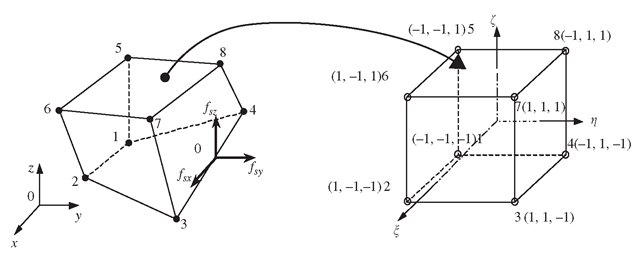
\includegraphics[width=\textwidth]{figures/FEmappingHex.png}
\end{frame}


\begin{frame}{Trilinear hexahedral element}
\centering
\begin{minipage}{0.6\textwidth}
    %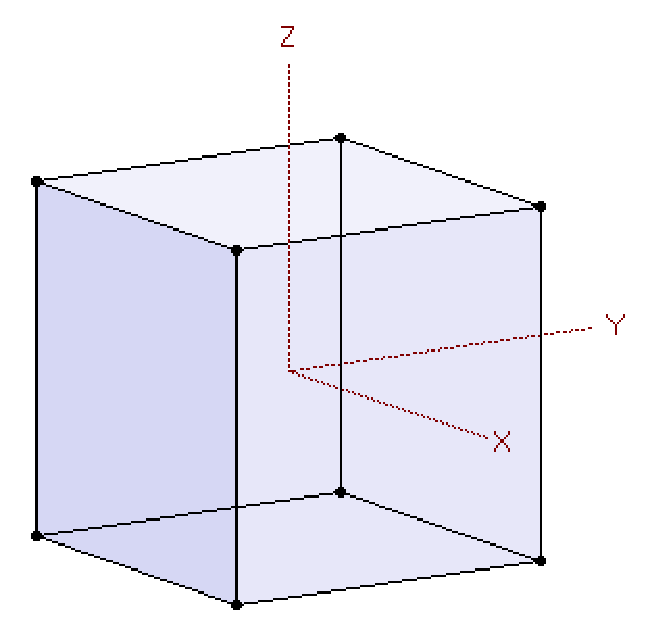
\includegraphics[width=0.9\textwidth]{figures/cubic.pdf}
    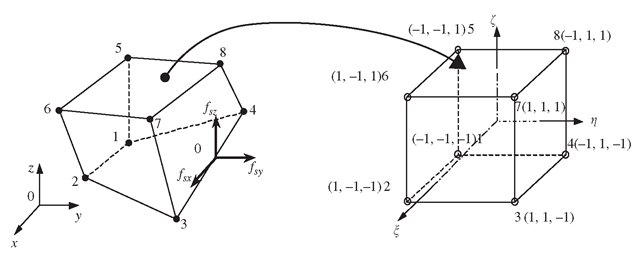
\includegraphics[width=\textwidth]{figures/FEmappingHex.png}
\end{minipage}
\begin{minipage}{0.35\textwidth}
{\scriptsize
\begin{align*}
N_1 &= \frac{1}{8}(1 - \xi)(1 - \eta)(1 - \zeta) \\
N_2 &= \frac{1}{8}(1 + \xi)(1 - \eta)(1 - \zeta) \\ 
N_3 &= \frac{1}{8}(1 + \xi)(1 + \eta)(1 - \zeta) \\
N_4 &= \frac{1}{8}(1 - \xi)(1 + \eta)(1 - \zeta) \\
N_5 &= \frac{1}{8}(1 - \xi)(1 - \eta)(1 + \zeta) \\
N_6 &= \frac{1}{8}(1 + \xi)(1 - \eta)(1 + \zeta) \\ 
N_7 &= \frac{1}{8}(1 + \xi)(1 + \eta)(1 + \zeta) \\
N_8 &= \frac{1}{8}(1 - \xi)(1 + \eta)(1 + \zeta) \\
N_i &= \frac{1}{8}(1 + \xi_i\xi)(1 + \eta_i\eta)(1 + \zeta_i\zeta)
\end{align*}
}
\end{minipage}

\end{frame}


\begin{frame}{3D integrals}
Gaussian quadrature in 1D: $n$ points can integrate exactly a polynomial
of degree equal to $2 n - 1$
\begin{align*}
I &= \int_{-1}^1 f(\xi) d \xi  \\
I &\approx \sum_{k=1}^n w_k f(\xi_k) \\
\end{align*}


Gaussian cubature
\begin{align*}
I &= \int_{-1}^1 \int_{-1}^1 \int_{-1}^1 f(\xi, \eta, \zeta) \; d \xi \; d \eta \; d  \zeta \\
I &\approx \sum_{k_1=1}^n \sum_{k_2=1}^n \sum_{k_3=1}^n w_{k_1} w_{k_2} w_{k_3} f(\xi_{k_1}, \eta_{k_2}, \zeta_{k_3}) \\
\end{align*}

\end{frame}

\begin{frame}{3D integrals $\ldots$}
Integrating the Laplacian on the reference element
\begin{align*}
I &= \int_{\Omega} \nabla N_i(x,y,z) \cdot \nabla N_j(x,y,z) d \Omega \\ \\
I &= \int_{\Omega_0} J^{-1} \nabla N_i (\xi, \eta, \zeta) \cdot J^{-1}\nabla N_j (\xi, \eta, \zeta) |J| d \Omega_0 \\ \\
I &= \int_{-1}^1 \int_{-1}^1 J^{-1} \nabla N_i(\xi, \eta, \zeta) \cdot J^{-1}\nabla N_j(\xi, \eta, \zeta) |J| d \xi \; d \eta \; d \zeta\\ \\
I &\approx  \sum_{k_1,k_2,k_3=1}^n  ( w_{k_1} w_{k_2} w_{k_3} J^{-1}_{k_1,k_2,k_3} \nabla N_i(\xi_{k_1}, \eta_{k_2}, \zeta_{k_3}) 
\\ & \cdot J_{k_1,k_2,k_3} \nabla N_j(\xi_{k_1}, \eta_{k_2}, \zeta_{k_3}) |J_{k_1,k_2,k_3}| ) \\
\end{align*}

\end{frame}


\begin{frame}{Fast Assembly using MATLAB}
\lstinputlisting[language=matlab,firstnumber=1,basicstyle=\ttfamily\scriptsize]{SuperFastAssembly.m}
\end{frame}

\begin{frame}{Fast Assembly of rhs using MATLAB}
\lstinputlisting[language=matlab,firstnumber=1,basicstyle=\ttfamily\scriptsize]{FastAssemblyRhs.m}
\end{frame}



\end{document}
